% this is the main tex document that compiles the text from each section file into one doc

% import packages to use in this template - DO NOT CHANGE ANYTHING BELOW THIS LINE
\documentclass[12pt, oneside]{book}
\usepackage[letterpaper, left=1.2in, right=1.2in, top=1.2in, bottom=1.2in]{geometry}
\usepackage{fancyhdr}
\pagestyle{plain}
\fancyhf{}
\renewcommand{\chaptermark}[1]{\markboth{\MakeUppercase{#1}}{}}
\usepackage{titlesec}
\usepackage{titletoc}
\usepackage{lipsum}
\titleformat{\chapter}[display] 
{\normalfont\huge\bfseries}{\chaptertitlename~\thechapter}{30pt}{\Huge}   
\usepackage{enumitem}
\usepackage{makecell}
\usepackage{float}
\usepackage{amsmath,amssymb,amsthm,amsfonts}
\usepackage{algorithmic}
\usepackage{graphicx}
\usepackage{booktabs, multirow} % for borders and merged ranges
\usepackage{tocloft}
\usepackage{tocbibind}
\usepackage{setspace}
\usepackage[utf8]{inputenc}
\usepackage[bookmarks=true, hidelinks]{hyperref}
\usepackage{natbib}

\setcounter{tocdepth}{2}
\setcounter{secnumdepth}{5}
\usepackage{titlesec}
\titlespacing*{\chapter}{0pt}{-30pt}{30pt}

\usepackage{graphics}
\usepackage{caption}
\usepackage{subcaption}
\usepackage{appendix}
\usepackage{listings}
\usepackage{bm}
\usepackage{lipsum}  

% some commands
\renewcommand{\cftchapfont}{\bfseries}
\renewcommand{\cftchappagefont}{\bfseries}
\renewcommand{\cftchapnumwidth}{1em}
\renewcommand{\cftchapdotsep}{\cftdotsep}
\renewcommand\cftchappagefont{\mdseries}
\renewcommand{\cftchapleader}{\cftdotfill{\cftchapdotsep}}
\renewcommand{\bibname}{Reference List}

\let\svthefootnote\thefootnote
\newcommand\freefootnote[1]{%
  \let\thefootnote\relax%
  \footnotetext{#1}%
  \let\thefootnote\svthefootnote%
}

\doublespacing
\begin{document}
%%%%%%%%%%%%%%%%%%%%%%%%%%%%%%%%%%%%%%%%%%%%%%%%%%%%%%%%%%%%%%%%%%%%%%%%%%%%%%%%%%%%%
% the sections below are what makes the final document -- see README

% title page and subsequent intro pages - EDIT VARIABLES AT THE TOP OF THIS DOCUMENT
% user defined variables
\newcommand{\docType}{thesis} % thesis or dissertation here -- NOT case sensitive
\newcommand{\yourDegree}{master of science} % e.g., Master of Science -- NOT case sensitive
\newcommand{\thesisTitle}{Examining Right-Moving Supercell Environments with Doppler Wind LiDAR Observations} % NOT case sensitive
\newcommand{\yourName}{Robert A Saba} % NOT case sensitive
\newcommand{\yourYear}{2024}
\newcommand{\academicUnit}{School of Meteorology} % NOT case sensitive
\newcommand{\yourMajor}{Meteorology} % NOT case sensitive

% committee members -- un-comment/comment out as needed here and in section beginning at line 82
\newcommand{\memberOne}{Dr. Michael Coniglio (Chair)} % keep (Chair) --> e.g., {Dr. John Doe (Chair)}
\newcommand{\memberTwo}{Dr. Stacey Hitchcock}
\newcommand{\memberThree}{Dr. Cameron Homeyer}
\newcommand{\memberFour}{Dr. Joshua Gebauer}
% \newcommand{\memberFive}{test}
% \newcommand{\memberSix}{test}

%%%%%%%%%%%%%%%%%%%%%%%%%%%%%%%%%%%%%%%%%%%%%%%%%%%%%%%%%
% Do not edit these lines unless you wish to customize the template (besides # of committee members)$
%%%%%%%%%%%%%%%%%%%%%%%%%%%%%%%%%%%%%%%%%%%%%%%%%%%%%%%%%

% begin the formatted title pages
\begin{titlepage}

% center subsequent text
\begin{center}

% hide page numbers for now
\pagenumbering{gobble}

% header
{\MakeUppercase{\large{University of Oklahoma\\Graduate College}}}

% space insert
\vspace*{4cm}

% title
\MakeUppercase{\thesisTitle} \\

% space insert
\vspace{2\baselineskip}
\vspace{3cm}

% add text
A \MakeUppercase{\docType}\\
SUBMITTED TO THE GRADUATE FACULTY \\
in partial fulfillment of the requirements for the\\
Degree of \\
\MakeUppercase{\yourDegree} \\
\MakeUppercase{(\yourMajor)} \\

% add text at the bottom of the page
\vfill
by \MakeUppercase{\yourName} \\
Norman, Oklahoma \\
\yourYear{}\\

% new page 
\newpage 

% vspace 
\vspace*{1cm}

% add text
\MakeUppercase{\thesisTitle} \\ 

% vspace 
\vspace*{1cm}

% add text
A \MakeUppercase{\docType} APPROVED FOR THE \\
\MakeUppercase{\academicUnit} \\

% vspace 
\vspace*{4cm}

BY THE COMMITTEE CONSISTING OF \\

% vspace 
\vspace{4cm}

% committee members -- un-comment/comment out as needed (must match the number provided at the top of doc)
\hfill\hfill \memberOne \\
\hfill\hfill \memberTwo \\
\hfill\hfill \memberThree \\
\hfill\hfill \memberFour \\
% \hfill\hfill \memberFive \\
% \hfill\hfill \memberSix \\

% new page for copyright -- at the bottom of the page 
\newpage
\vspace*{\fill}

\textcopyright Copyright by \MakeUppercase{\yourName} \yourYear \\
All Rights Reserved.

\end{center}
\end{titlepage}

% Acknowledgements - PAGE NUMBERING STARTS HERE (IN ROMAN NUMERALS)
\pagenumbering{roman}
\addcontentsline{toc}{chapter}{Acknowledgments}
\setcounter{page}{4} 
% format the chapter/section details
\chapter*{Acknowledgments}

% insert your text below the line
%-------------------------------------------
your acknowledgments here

\clearpage

% Table of Contents
\renewcommand\contentsname{Table of Contents}
\addtocontents{toc}{\protect\setcounter{tocdepth}{-1}}
\begin{singlespace}
    \setlength\cftbeforetabskip{\baselineskip}
    \tableofcontents
\end{singlespace}
\addtocontents{toc}{\protect\setcounter{tocdepth}{2}}
\clearpage

% List of figures and tables
\begin{singlespace}
    \setlength\cftbeforetabskip{\baselineskip}
    \listoftables
\end{singlespace}
\clearpage

\begin{singlespace}
    \setlength\cftbeforefigskip{\baselineskip}
    \listoffigures
\end{singlespace}
\clearpage

% Abstract
% format the chapter/section details
\chapter*{Abstract}
\chaptermark{Abstract}
\label{chap:Abstract}
\addcontentsline{toc}{chapter}{Abstract}

% insert your text below the line
%-------------------------------------------
While immense enhancements to meteorological observations and simulations have been made over the last several decades, two lingering questions continue to plague the community: (1) Why do some storms produce tornadoes while others do not, and (2) why do storms in seemingly identical environments go on to produce different hazards? Developing robust answers to these questions are critical as tornadoes continue to be a top cause for weather-related fatalities. Storm environment research through simulated storms, reanalysis products, and limited observations have guided the current understanding and have identified differences between environments supportive of tornadic and non-tornadic supercells. This work aims to use more detailed observations through Doppler wind lidars to capture the storm environment evolution in both time and space. 

Since 2016, the National Severe Storms Laboratory has operated mobile scanning Doppler wind lidars within the inflow of supercell thunderstorms as part of collaborative field projects (mini-MPEX, TORUS, PERiLS, TORUS-LiTE, and LIFT). The research goal of this instrument is to observe the evolution of storm inflow properties to gain a better understanding of the storm environment surrounding an evolving supercell. Various scanning and post-processing techniques to capture the wind profile evolution via DWL observations have been used. Prior to 2022, a velocity azimuth display technique was used to retrieve a vertical wind profile every 3-5 minutes using 8 points 20 degrees off zenith.  In 2022-23, a continuous scanning mode was implemented to retrieve wind profiles as frequent as every 5 seconds. Both of these scanning strategies yielded vertical profiles of derived horizontal winds about every 18 meters with the first usable data point around 75 meters AGL after filtering based on a signal-to-noise ratio threshold. A new optimal estimation technique was designed to incorporate co-located rawinsonde and surface observations into the wind retrievals that provide data between the surface and 75 meters. These observations are used to validate the post processing techniques and output will be compared to previously used methods.

Focus will be placed on the evolution of the near-ground kinematic characteristics and the storm induced environmental modification in both tornadic and non-tornadic storms. To remove background trends from the environmental evolution, Rapid Refresh model-based analysis profiles are used. Full, surface-based wind profiles will allow for the quantification and time evolution of severe weather forecasting parameters, such as storm-relative helicity, storm-relative winds, etc. Implications of these results on recent studies discussing the relative importance of streamwise vorticity versus storm-relative winds on supercell properties and tornado production will be discussed. 

Results show that differences in mesocyclone intensity between tornadic and non-tornadic supercells cause the downstream spatial variability of their environments. This is particularly true when quantifying storm-induced accelerations, which can lead to the length scales at which mesocyclone induced perturbations can be observed. Furthermore, low-level ground-relative winds tend to provide greater differences in the storm environment whereas storm-relative winds contain greater composite differences above 1 kilometer. Also explored are the vorticity trends in these storm environments in time and space, and the horizontal vorticity components (and associated differences) will be shown. 






\clearpage

%%%%%%%%%%%%%%%%%%%%%%%%%%%%%%%%%%%%%%%%%%

% resume page numbering for rest of document
\pagenumbering{arabic}
\setcounter{page}{1} % set the page number appropriately

% Chapter 1
% format the chapter/section details
\chapter{Introduction}
\label{chap:intro}

% contained in this file are examples for inserting figures, tables, and equations as well as in text citations
% % figure example 
% \begin{figure}[h!]
%     \centering % center the graphic in the text
%     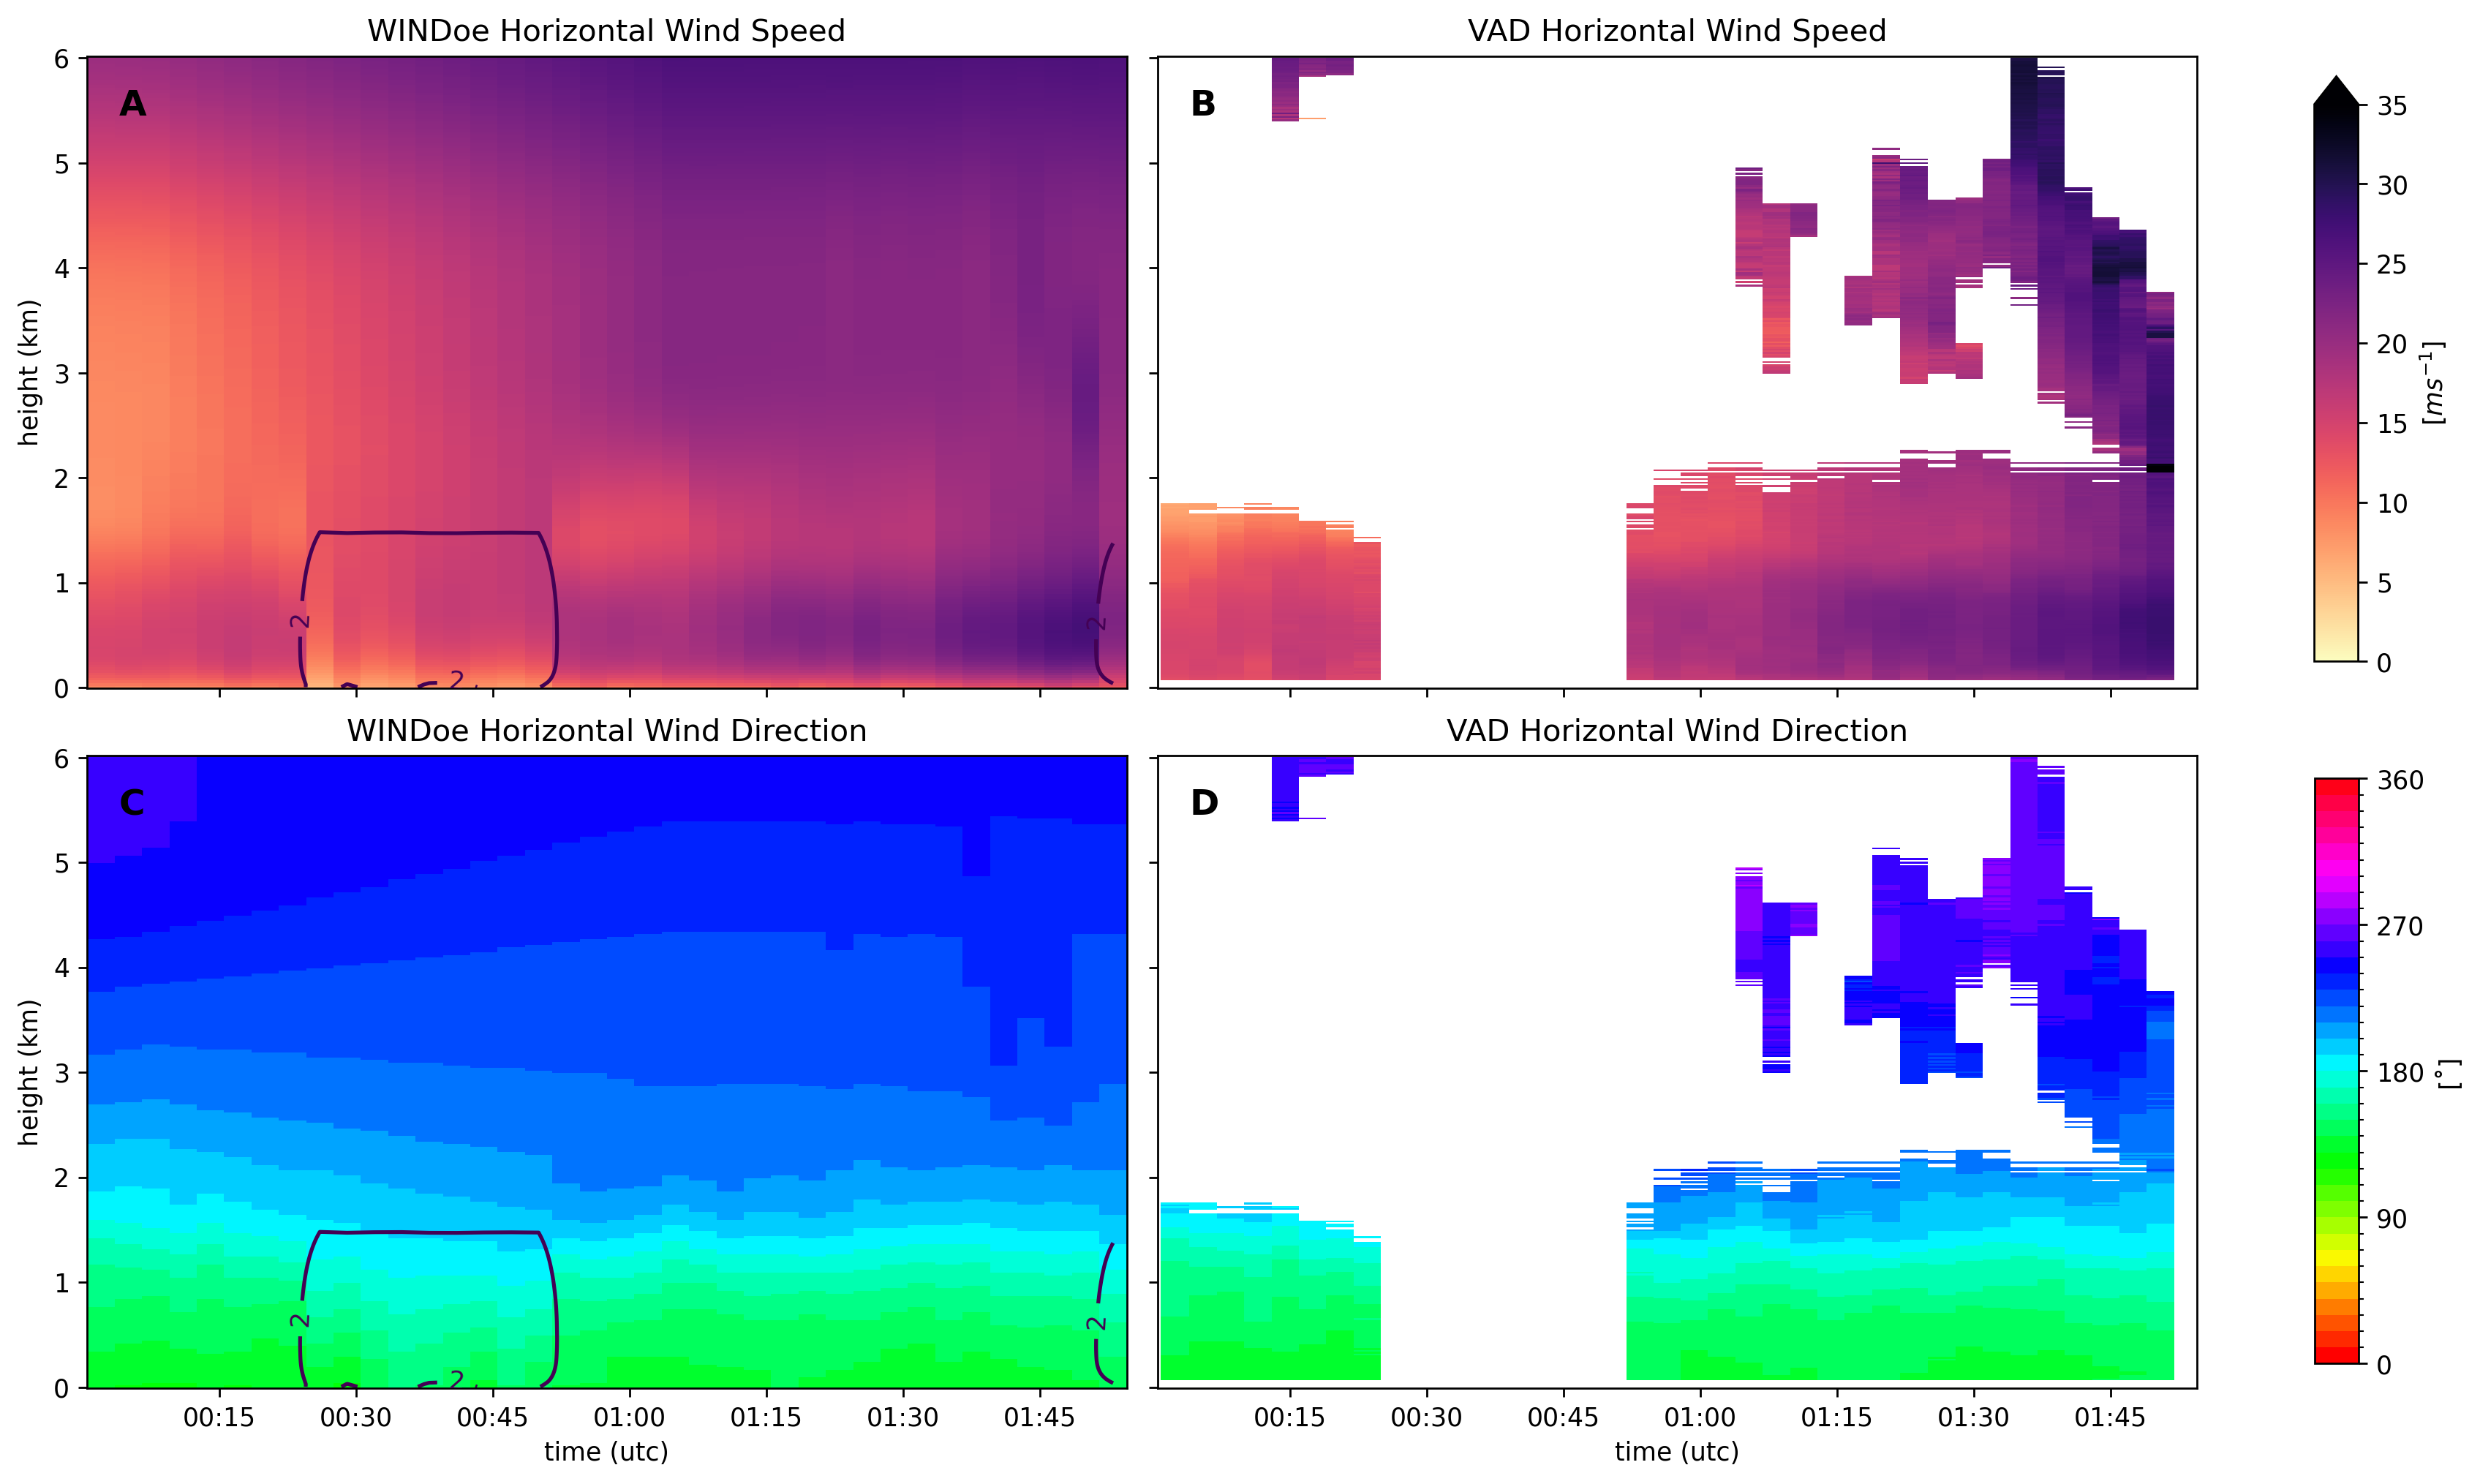
\includegraphics[width=0.7\textwidth]{figures/example.png} % include the figure
%     \caption{some caption} % add a caption
%     \label{fig:some_fig} % label the figure for referencing in the paper
% \end{figure}

% % equation example 
% \begin{equation}
%     \omega_h = (\frac{dw}{dy} - \frac{dv}{dz}, \frac{du}{dz} - \frac{dw}{dx}) % add equation
%     \label{eq:some_eq} % label equation for referencing in paper
% \end{equation}

% % table example
% \begin{table}[h!]
%     \centering % center the table in the text
%     \begin{tabular}{c|c|c} % begin the table with the text orientation of the text in table cells
%         \textbf{variable} & \textbf{variable 2} & \textbf{variable 3} \\\hline % headers
%         test & test & test\\ % values (this is one row)
%         test & test & test\\ % values (this is one row)
%         test & test & test\\ % values (this is one row)
%     \end{tabular}
%     \caption{some caption} % add a caption
%     \label{tab:some_table} % label table for referencing in paper
% \end{table}

% % in text citation example 
% when using this template, please use /citep{} for in text citations (e.g. \citep{smith2020}) and \cite{} for in 
% text citations that are part of the sentence (e.g. \cite{smith2020} found that...)

% insert your text below the line
%-------------------------------------------
A better understanding of supercell thunderstorms and their hazards is critical towards saving a disproportionate number of lives lost compared to other weather-related events \citep{brotzge2013tornado}. Efforts continue in both modeling and observational research to decipher differences between various supercell environments and the downstream hazards associated with storms within them \cite[e.g.,][]{nowotarski2013classifying, parker2014composite, coffer2020near, coniglio2020insights}. Of note, predicting tornadic versus non-tornadic supercells has been particularly difficult \citep{brooks2018long}. These difficulties highlight the importance of storm environment research and developing a better understanding of storm environment variability.

\section{Supercell Thunderstorms}
The term 'supercell' is used to describe a thunderstorm with a rotating updraft, or mesocyclone \citep{browning1962sup}. An early distinction found between supercells and ordinary thunderstorms was their movement separate from the mean wind. \cite{browning1964airflow} created a formal model of the now coined, 'right moving supercell'. As time and research progressed, a supercell was used to describe an anti-cyclonically rotating storm moving to the left or a cyclonically rotating storm moving right of the mean wind. In this study, only right-moving supercells are analyzed. Schematics for these storms were developed by \cite{lemon1979severe} who posed a two dimensional view of supercell structure and it's governing features (Fig. \ref{fig:sup2d}) as well as an evolutionary diagram of the supercell and its associated updraft and downdraft evolution (Fig. \ref{fig:supevolution}). 

\begin{figure}[h!]
    \centering
    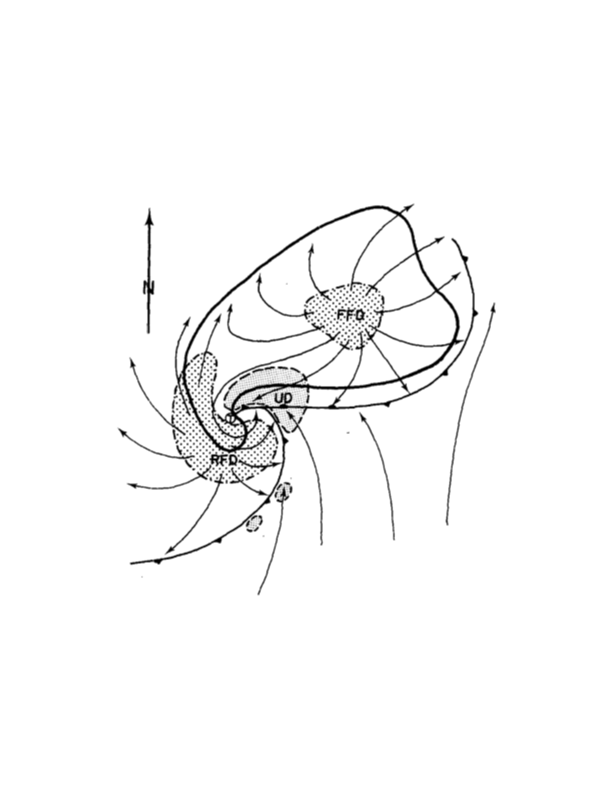
\includegraphics[width=1\textwidth]{figures/supercell_2d.png}
    \caption{One of the first two dimensional views of a supercell and its primary regions. Regions include the forward and rear flank downdraft (FFD/RFD), updraft (UD), and a generalized flow pattern. Figure from \cite{lemon1979severe}. Their figure 7.}
    \label{fig:sup2d}
\end{figure}

\begin{figure}[h!]
    \centering
    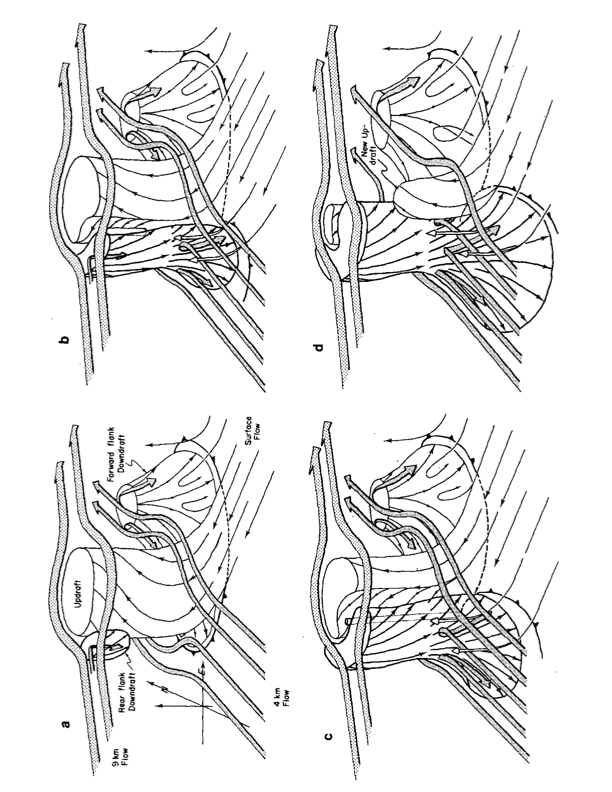
\includegraphics[width=0.75\textwidth, angle = 270]{figures/supercell_evolution.png}
    \caption{Updraft and downdraft evolution during the lifetime of a supercell thunderstorm including mid and upper level flow patters and previously identified storm features. Figure from \cite{lemon1979severe}. Their figure 9.}
    \label{fig:supevolution}
\end{figure}


% Chapter 2
% format the chapter/section details
\chapter{Data and Methods}
\label{chap:data_methods}

% insert your text below the line
%-------------------------------------------
text here

% Chapter 3
% format the chapter/section details
\chapter{Results}
\label{chap:results}

% insert your text below the line
%-------------------------------------------
This chapter addresses the results from this study as they relate to each of the hypotheses in chapter \ref{chap:intro}. Additional results as they were made apparent in the data will be discussed thereafter.

\section{Hypothesis Driven Results}
\subsection{Environmental Spatial Variabilities}
Previous observational based efforts have found greater spatial variability in non-tornadic inflow environments compared to tornadic storm environments \citep{parker2014composite}. Given their dataset of rawinsonde launches, these variances were displayed through SRH and composite wind profiles (Fig. \ref{fig:parker_comp}). Using similar methodology, we can assess this dataset in a near and far-field perspective. First, an assessment of the number of profiles making up each spatial bin must be addressed (Fig. \ref{fig:space_nprofs}). Composite profiles can then be created showing near and far-field hodographs in tornadic and non-tornadic storms (Fig. \ref{fig:inflow_hodos}). In this work, the near-field will be used to describe the inflow environment up to 30 kilometers away in the x-direction. Far-field will consist of data beyond the 30 kilometer threshold. 

\begin{figure}[h!]
    \centering
    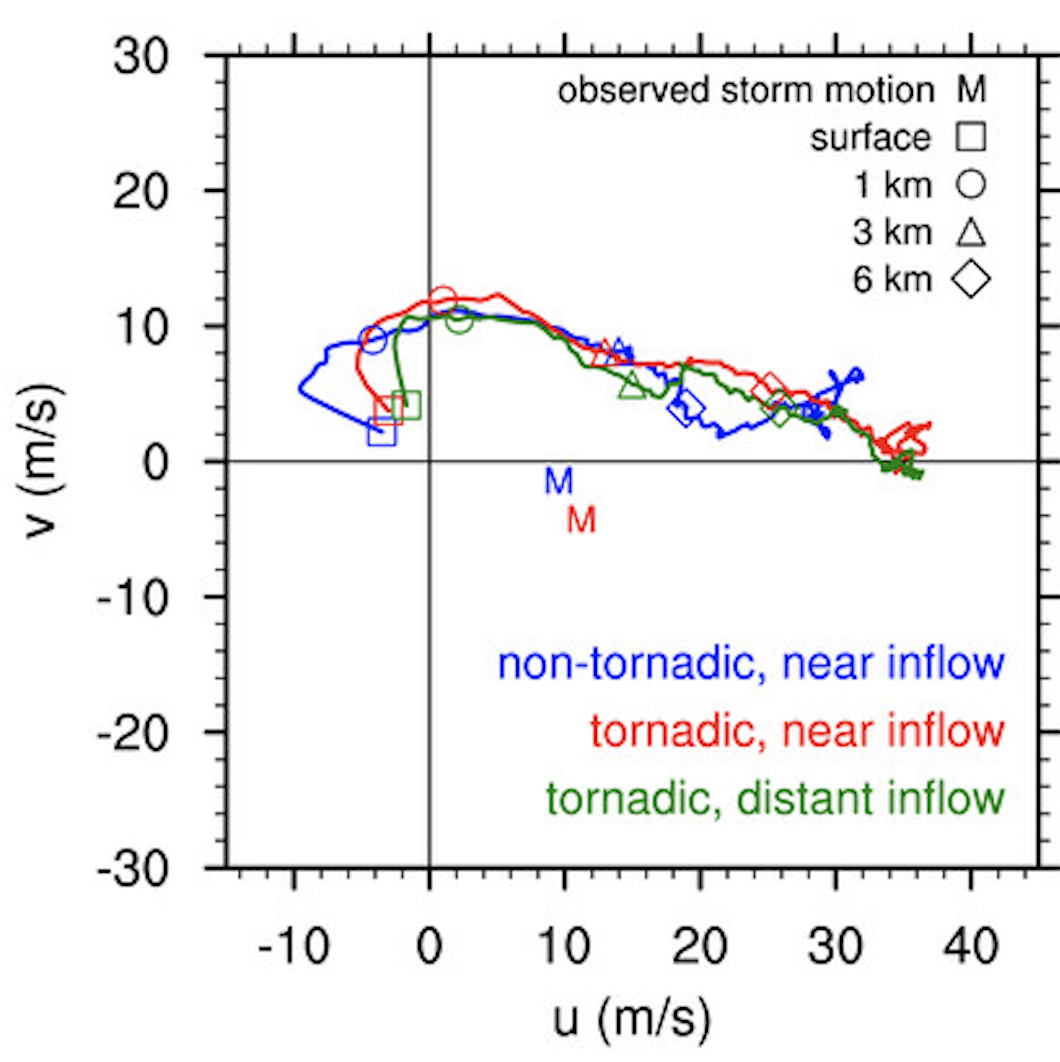
\includegraphics[width = 1\textwidth]{Figures/parker_composite.png}
    \caption{VORTEX-2 composite wind profiles, drawn from rawinsonde launches. From \cite{parker2014composite}; their figure 12.}
    \label{fig:parker_comp}
\end{figure}

\begin{figure}[h!]
    \centering
    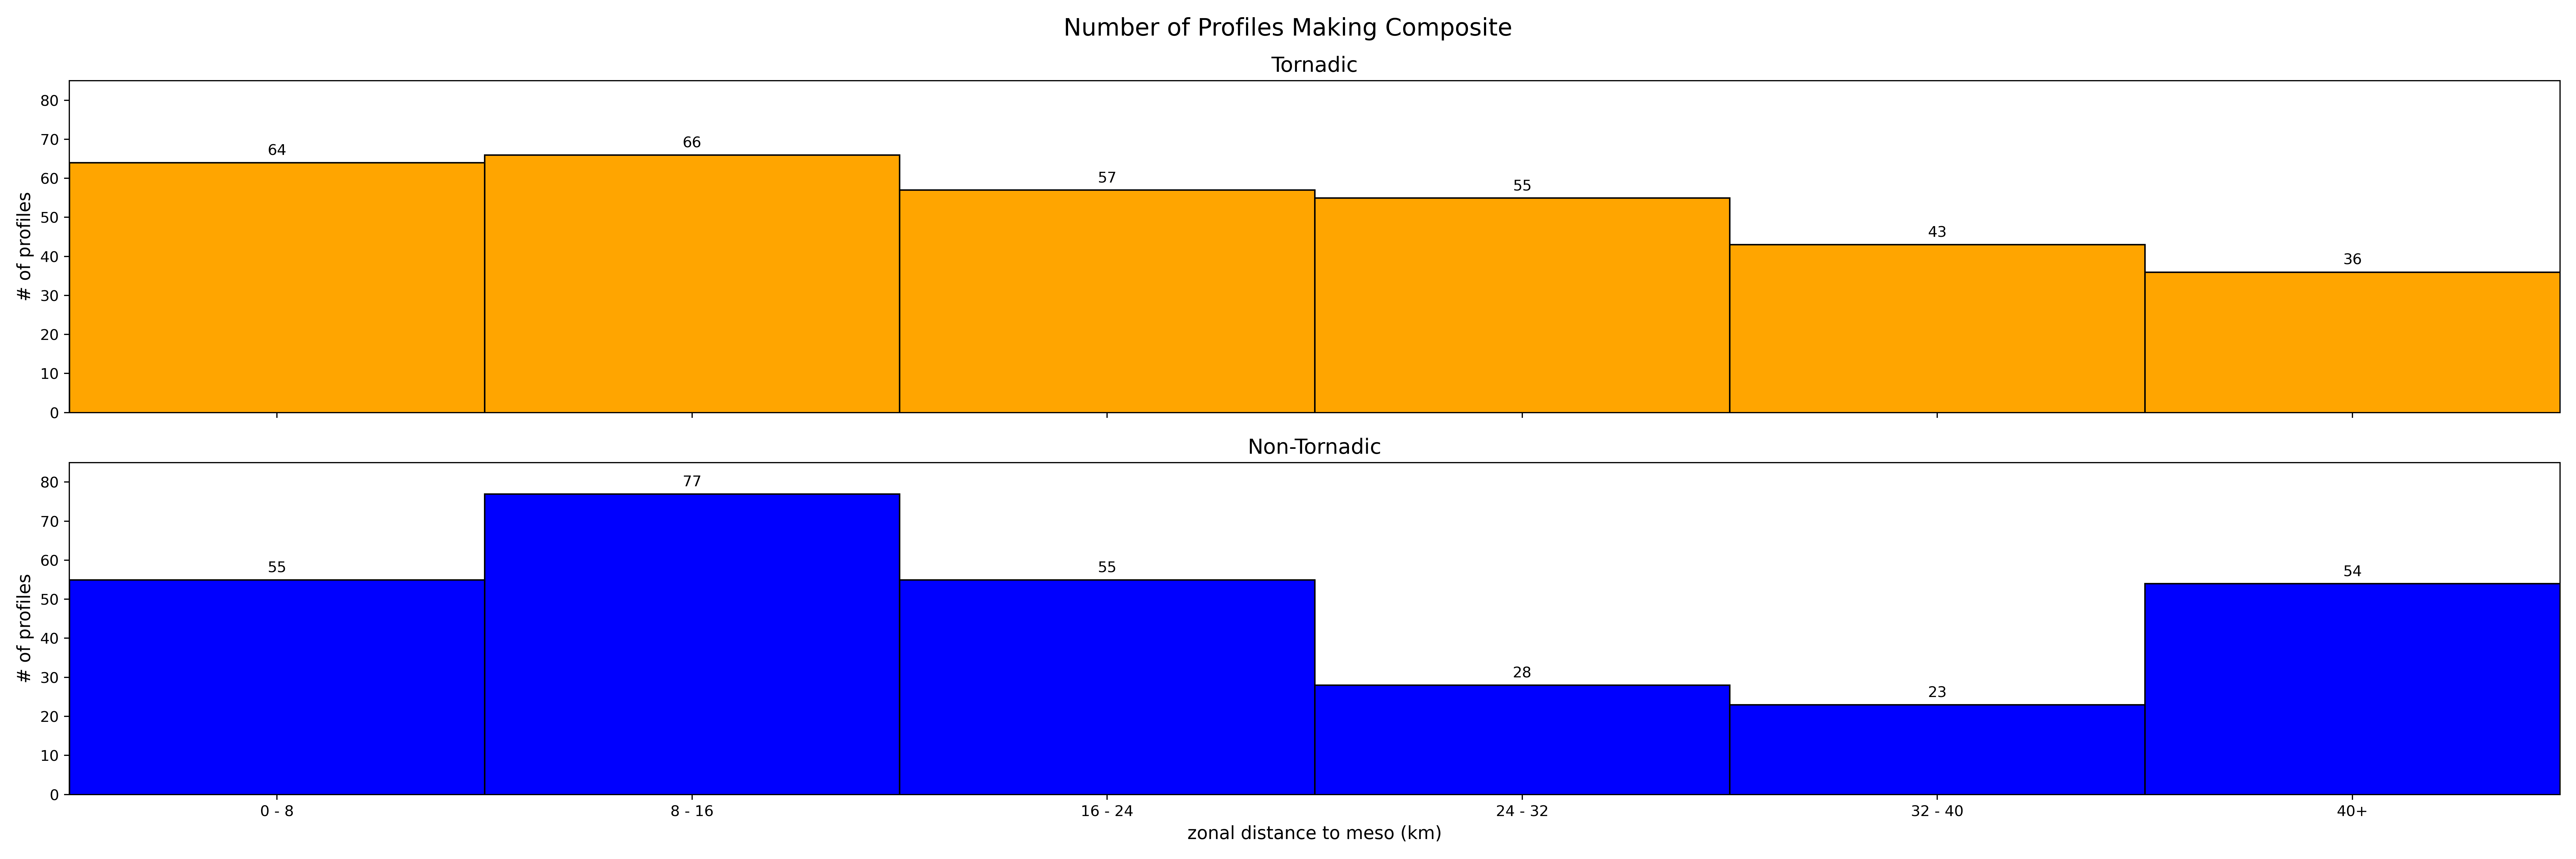
\includegraphics[width = 1\textwidth]{Figures/spatial_nprofs.png}
    \caption{Histogram of the number of WINDoe profiles making up the spatial composites used in this section. Counts for tornadic (top, orange) and non-tornadic (bottom, blue) composites are shown.}
    \label{fig:space_nprofs}
\end{figure}

\begin{figure}[h!]
    \centering
    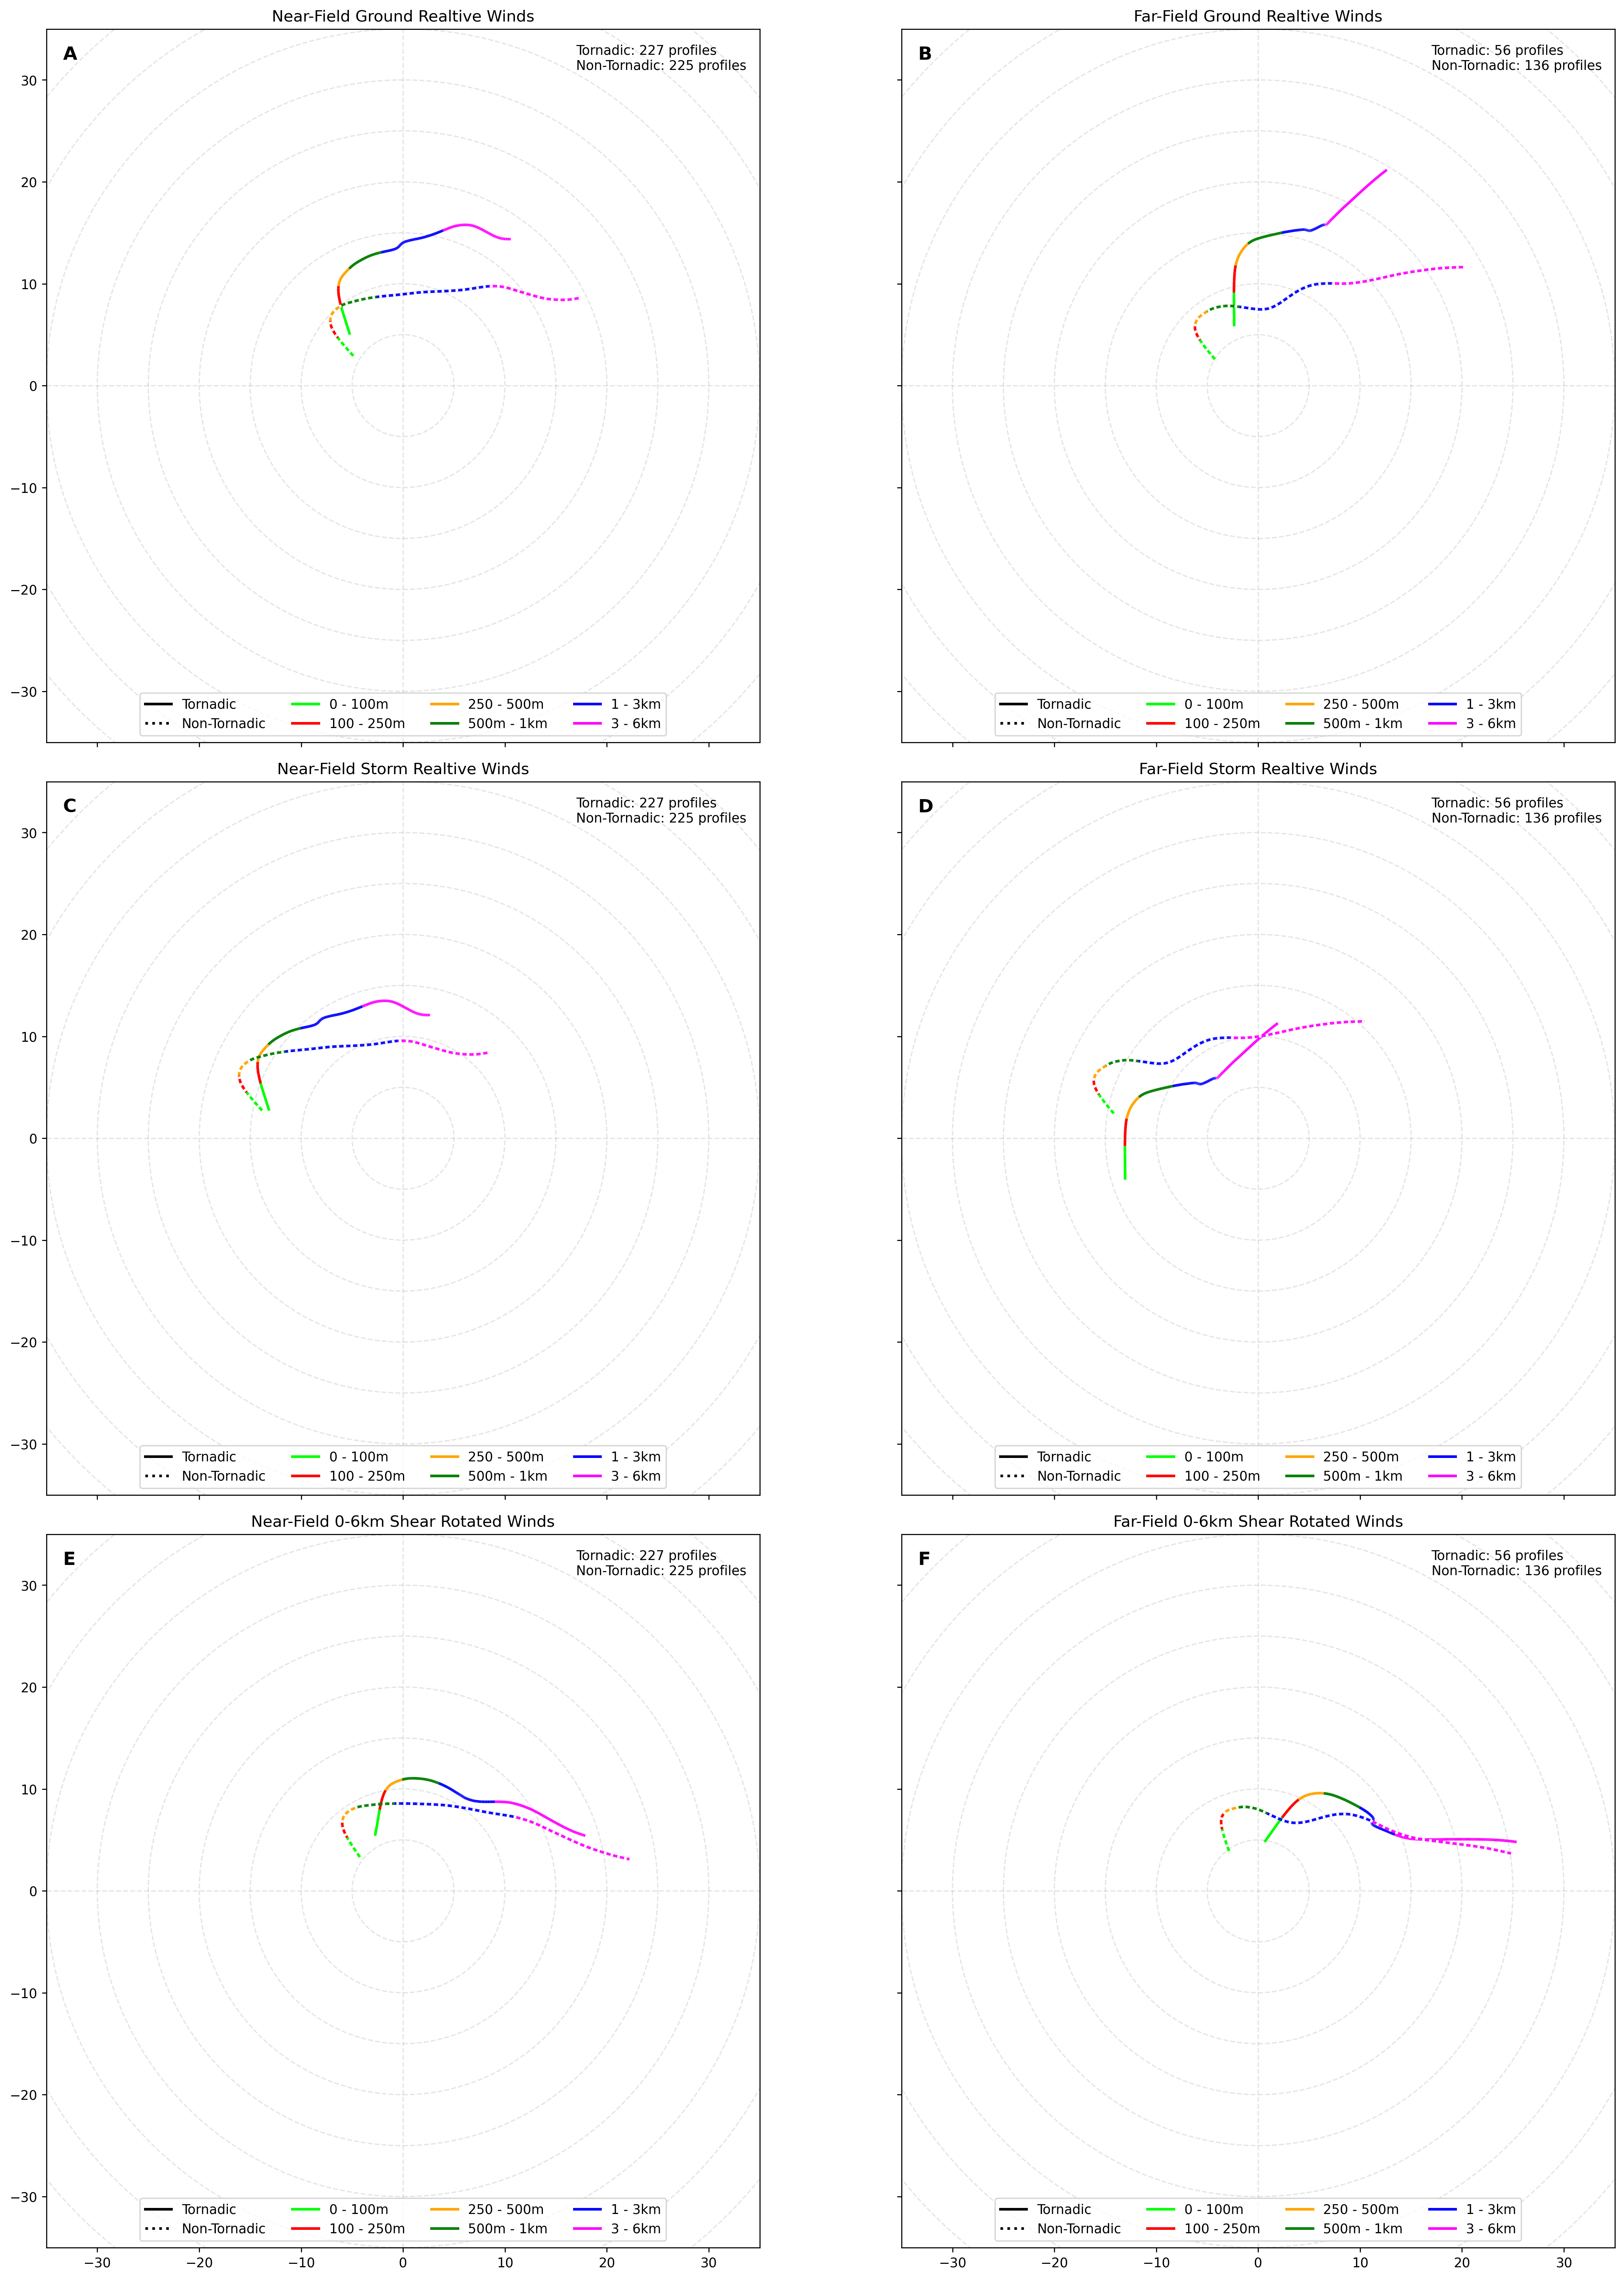
\includegraphics[width = 0.8\textwidth]{Figures/inflow_hodos_tor_no_neg.png}
    \caption{Composite ground relative (A,B; $ms^{-1}$), storm relative (C,D; $ms^{-1}$), and 0-6km shear vector rotated (E,F; $ms^{-1}$) hodographs for near-field and far-field inflow regions. Tornadic (solid) and non-tornadic (dashed) profiles are shown with the number of profiles comprising each composite shown in the respective panel.}
    \label{fig:inflow_hodos}
\end{figure}

% Chapter 4
% format the chapter/section details
\chapter{Summary and Conclusions}
\label{chap:discussion}

% insert your text below the line
%-------------------------------------------
To this point in severe storms research, the use of DWL data in convective environments has been minimal. This work provides an atypical use case for the instrument and displays the benefits of using an instrument of this nature to observe severe convective storm environments, particularly in detailing the near-ground wind profiles. Although the main drawback of using DWLs for this purpose lies in their blind spot below  about 60 to 80 meters, improvements to post-processing techniques have aided in alleviating this problem. In this study, we have explored the use of DWL wind retrievals and a wind estimation method (WINDoe) to quantify the evolution and variability of the low-level wind profile in storm environments. Specifically using the prior dataset created for use in this analysis, WINDoe provides an opportunity to combine DWL wind retrievals with other observational data sets to create a unified analysis of the wind profile over the lower troposphere in severe storm environments. Furthermore, WINDoe quantifies uncertainty in the retrievals, something missing from many observational based studies to this point in the science. Overall, the ability for this instrument to be nimble in operational settings, tied together with strides in data-analysis techniques should highlight the possibilities of utilizing DWLs in severe storms research.

This research provides an in-depth observation-based analysis into how supercell storm environment wind profiles evolve in time and space exploiting the ability of DWLs to retrieve wind profiles as frequently as every 5-10 seconds with high vertical resolution (about 18 meters). This includes the environmental differences between tornadic and non-tornadic storm environments, building on a lengthy literature of storm environment research rooted in observations, reanalysis, and simulated storms. Many previous efforts have yielded conflicting results, so this work seeks to provide clarity through the use of real-world datasets while targeting the most intense non-tornadic storms, findings that could further inform the forecasting community. Based on previous efforts this work addressed the following hypotheses:

\begin{enumerate}
    \item Kinematics vary more in non-tornadic storms in space, with drastic changes in SRH from the far-field to near-field not seen in tornadic composites \citep{parker2014composite}. 
    \item Low-level, inflow winds in non-tornadic supercell environments contain more crosswise vorticity compared to their tornadic supercell counterparts \citep{parker2014composite}.
    \item SRW plays an insignificant role in tornado dynamics and thus, there are minimal differences in low-level SRW profiles in tornadic and non-tornadic environments \citep{peters2023disentangling}.
    \item Streamwise vorticity drives changes in SRH in the storm environment and provides the skill between SRH and tornado prediction \citep{peters2023disentangling}.
    \item Low-level parameters such as SRH$_{500m}$ provide better discriminatory skill compared to deeper-layer parameters such as SRH$_{1km}$ or SRH$_{3km}$ \citep{coffer2019using, coniglio2020insights}.
\end{enumerate}

% % Chapter 5 - uncomment out as needed
% % format the chapter/section details
% \chapter{Future Directions}
% \label{chap:future directions}

% insert your text below the line
%-------------------------------------------

% \clearpage

% % Appendices - uncomment out as needed
% % format the chapter/section details
\begin{appendices}

\addtocontents{toc}{\protect\renewcommand{\protect\cftchappresnum}{\appendixname\space}}
\addtocontents{toc}{\protect\renewcommand{\protect\cftchapnumwidth}{6em}}

\chapter{Appendix A}
% insert your text below the line
%-------------------------------------------

\end{appendices}

% bibliography
%========================================
\begin{singlespace}
    \setlength\bibsep{\baselineskip}
    \bibliographystyle{ametsocV6}
    \bibliography{Reference}
\end{singlespace}

% end doc
\end{document}